\documentclass[amssymb,twocolumn,aps]{revtex4}

% allows special characters (including æøå)
\usepackage[utf8]{inputenc}
%\usepackage [norsk]{babel} %if you write norwegian
\usepackage[english]{babel}  %if you write english

\usepackage{physics,amssymb}  % mathematical symbols (physics imports amsmath)
\usepackage{graphicx}         % include graphics such as plots
\usepackage[table]{xcolor}
\usepackage{xcolor}           % set colors
\usepackage{hyperref}         % automagic cross-referencing 
\usepackage{float}			  % force placement of tables and figures

\begin{document}
	
\title{Report Template \\
    \normalsize FYS-STK3155 - Project X}
\date{\today}               
\author{Student}
\affiliation{University of Oslo}

\newpage
	
\begin{abstract}

A study of various regression methods, including OLS, Ridge and LASSO and how they fit Runge's function. We go through the theory and implementation of these methods and see how they compare on the function. In the end, we go through some resampling techniques on the simpler OLS-method to understand the bias-variance trade-off.
\end{abstract}

\maketitle

\section{Introduction}

The fundamental challenge in machine learning and statistical modeling is to extract meaningful patterns from data to build models that can make accurate predictions on new, unseen data. A simple approach might fit the training data perfectly, yet fail spectacularly when facing new instances—a phenomenon known as overfitting. Conversely, a model that is too simple may fail to capture the underlying structure of the data, leading to underfitting. This delicate balance is often described by the bias-variance tradeoff, a central concept in statistical learning that quantifies this tension between model simplicity and complexity \cite{hastie}. Effectively navigating this tradeoff is paramount for developing robust and generalizable models. This project delves into this core problem through the lens of regression analysis, a cornerstone of supervised learning used to predict continuous outcomes \cite{compfys}.

To investigate these principles, this report presents a comparative study of three fundamental regression methods: Ordinary Least Squares (OLS), Ridge, and Least Absolute Shrinkage and Selection Operator (LASSO) regression. We apply these methods to a specific one-dimensional problem: fitting a polynomial model to Runge's function, $f(x)=1/(1+25x^2)$. This function is notoriously difficult for high-degree polynomial interpolation, making it an excellent candidate for demonstrating the pitfalls of overfitting and the benefits of regularization techniques like Ridge and LASSO \cite{hein}. By analyzing model performance through metrics like Mean Squared Error (MSE) and the R2 score, we explore how each method handles increasing model complexity. Furthermore, we implement and analyze resampling techniques—specifically bootstrap and k-fold cross-validation—to empirically study the bias-variance tradeoff in the context of our OLS models.

The report is structured as follows. Section 2 establishes the theoretical framework, detailing the mathematical formulations of OLS, Ridge, and LASSO regression. This section also includes a formal derivation of the bias-variance decomposition of the MSE. Section 3 outlines the computational methodology, including the generation of our dataset from Runge's function, the implementation of the regression algorithms, and the setup for the resampling procedures. Section 4 presents and discusses the results of our numerical experiments, comparing the performance of the different regression methods and visualizing the bias-variance tradeoff as a function of model complexity. Finally, Section 5 provides a summary of our findings and concluding remarks on the relative strengths and weaknesses of each approach.


When you write the introduction you should focus on the following aspects:
\begin{itemize}
    \item Motivate the reader, the first part of the introduction gives always a motivation and tries to give the overarching ideas. Citing some central ideas or problems in the literature is a good idea here. \cite{compfys}\cite{eigenvalue}\cite{hein, hastie}
    \item What you have done, with a focus on choice of problem and method, and why these were chosen.
    \item The structure of the report, how it is organized. List the sections, and very briefly describe what is in them and how they fit together.
\end{itemize}
    
\section{Methods}\label{section:methods}

\subsection{Method 1/X}

\begin{itemize}
    \item Describe the methods and algorithms, including the motivation for using them and their applicability to the problem
    \item Derive central equations when appropriate, the text is the most important part, not the equations.
\end{itemize}

\subsection{Implementation}

\begin{itemize}
    \item Explain how you implemented the methods and also say something about the structure of your algorithm and present very central parts of your code, not more than 10 lines
    \item You should plug in some calculations to demonstrate your code, such as selected runs used to validate and verify your results. A reader needs to understand that your code reproduces selected benchmarks and reproduces previous results, either numerical and/or well-known closed form expressions.
\end{itemize}

\subsection{Use of AI tools}
	
\begin{itemize}
    \item Describe how AI tools like ChatGPT were used in the production of the code and report.
\end{itemize}
	
\section{Results and Discussion}\label{section:results} 
Below you see a picture that describes the Bias-Variance Trade off, \ref{fig:BiasVariance1}. The trade off here is visualized by having a model of higher complexity molding more and more to the training set thereby having a better fit or bias, but a worse fit on the unseen data.


\begin{itemize}
    \item Present your results
    \item Give a critical discussion of your work and place it in the correct context.
    \item Relate your work to other calculations/studies
    \item An eventual reader should be able to reproduce your calculations if she/he wants to do so. All input variables should be properly explained.
    \item Make sure that figures\ref{fig:BiasVariance1} and tables contain enough information in their captions, axis labels etc. so that an eventual reader can gain a good impression of your work by studying figures and tables only.
\end{itemize}

\begin{figure}[h]
    \centering
    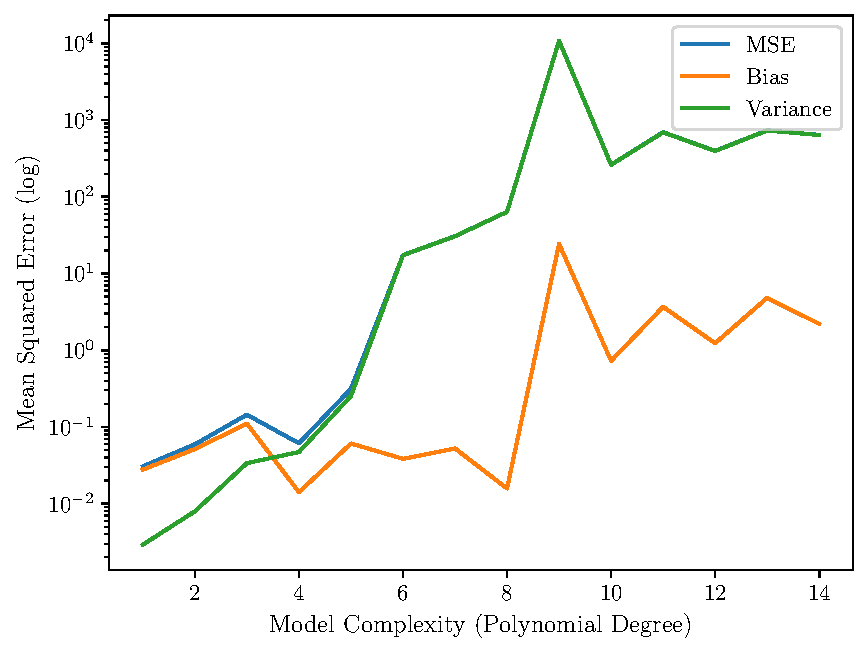
\includegraphics[width=0.9 \linewidth]{Figures/bias_variance_tradeoff.pdf}
    \caption{Bias Variance Tradeoff}
    \label{fig:BiasVariance1}
\end{figure}


\begin{figure}[h]
    \centering
    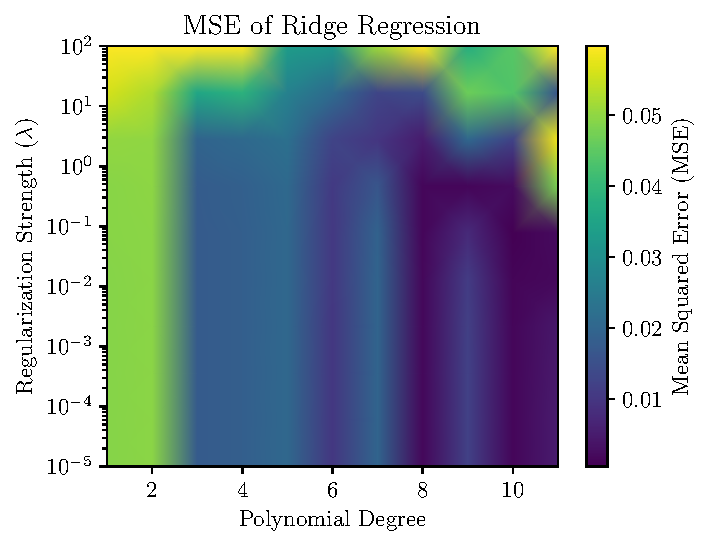
\includegraphics[width=0.9 \linewidth]{Figures/ridge_heatmap.pdf}
    \caption{Degree and Regularization Heatmap}
    \label{fig:DegRegHeat}
\end{figure}
The following heatmap, \ref{fig:DegRegHeat}, implies that a polynomial degree of around 5-6 and a regularization value of about $10^{-2} \lambda$ would be the best parameters for trainign the model.
\section{Conclusion}\label{section:conclusion} 
\begin{itemize}
    \item State your main findings and interpretations
    \item Try to discuss the pros and cons of the methods and possible improvements
    \item State limitations of the study
    \item Try as far as possible to present perspectives for future work
\end{itemize}

\bibliography{biblio}

\end{document}
